\documentclass[main.tex]{subfiles}
\begin{document}

\section{Example Robot Programs}
The following example robot programs make use of the Aria and MobileSim
softwares. The source code can be found in~\apref{appendA}.

\subsection{Aria Basics}

Aria\footnote{\url{http://robots.mobilerobots.com/Aria/docs/main.html}} is an
SDK framework written in C++ for controlling mobile robots. It aims to free the
programmer from low level tasks (such as signal processing, motor code, and
interrupts) to allow for higher level control methods.  \figref{ariaCtrl} shows
an overview of the control system that is implemented.  Essentially the robot
runs its own firmware that is in charge of low level commands (gathering sensor
data, direct motor control, etc.) which communicates with a server. The server
performs higher level data analysis and control methods. 

The server handles control methods via control commands. That is there is a
series of low level commands that the server communicates to the robot. These
low level commands can then be abstracted into higher level motion commands.
Motion commands are used to command the robot to perform motion actions such as
driving a certain distance or rotating at a certain speed. These commands are
converted into low level commands at run time.

Motion commands are also abstracted into what Aria calls Actions. Actions are
thought of as modules composed of motion commands that can be connected together
to achieve more complex motion. Each action has a set of motion commands it uses
to perform a desired action (such as avoiding a wall, or moving forward at a
constant velocity).  The Actions are added to a list and are evaluated upon
runtime to produce a series of low level commands. Each Action is given a weight
when added to the action list. This allows for prioritizing of actions and so
the actions with higher priority have more influence on the outcome of the robot
commands.

Each action can be thought of as running in parallel to the main server code and
other actions. This becomes important in the S-curve program where the robot is
commanded to go to a position once it has reached a certain location. Because
actions are used these commands are independent of one another and the robot can
handle internally when to obey the given commands. 

\begin{figure}[H]
\begin{center}
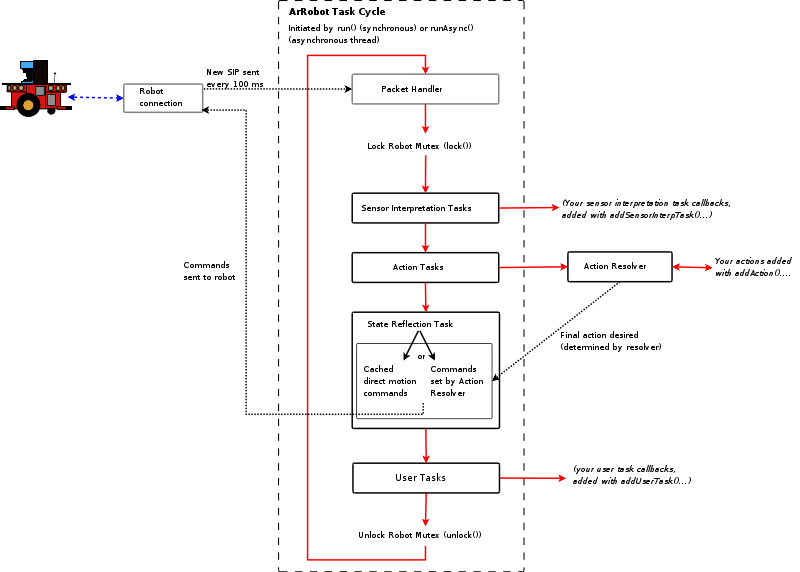
\includegraphics[width=.5\textwidth]{ArRobot_Task_Cycle}
\end{center}
\caption{Aria Control System Overview}
\label{fig:ariaCtrl}
\end{figure}

\subsection{Square Path Robot}
The square robot program is a basic program that drives a robot in a square
path. Each side of the square is two meters long and the goal was simply to
drive this path as accurately as possible. The algorithm used to travel the
square path is show in \alref{alg1}. 

An Aria action class is used to drive the robot towards the desired goal. It
continuously monitors its position and rotates the robot to face the goal so as
to make it drive in a straight line (the robot will not drive straight until it
is fully rotated towards the desired location). \alref{alg1} and
\alref{driveStraight} run concurrently in software thus the robot will go
towards the desired goal once it has been commanded.

\begin{algorithm}
\caption{Procedure for Navigating a Square Path}
\label{al:alg1}
\begin{algorithmic}
	\FOR{$i=0$ to $3$}
		\STATE set the next robot position 
		\WHILE{robot has not reached desired goal}
			\STATE nothing
		\ENDWHILE
	\ENDFOR
\end{algorithmic}
\end{algorithm}

\newcommand{\delxi}{\Delta\xi}

\begin{algorithm}
\caption{Drive Straight Towards Goal}
\label{al:driveStraight}
	\begin{algorithmic}
		\IF{$\theta - \theta_{Goal} > 0$}
			\STATE rotate towards goal
			\STATE set translational velocity to 0
		\ELSIF{robot is not within goal threshold}
			\STATE drive robot towards goal
		\ENDIF
	\end{algorithmic}
\end{algorithm}

\begin{figure}[H]
	\begin{center}
	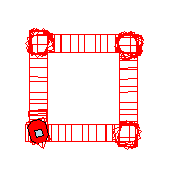
\includegraphics[]{squareBot}
	\end{center}
	\caption{Square Robot Path}
	\label{fig:sqBotPath}
\end{figure}

\figref{sqBotPath} shows the result of the square robot simulation. The red
boxes are the locations of the robot at certain time frames; it can be viewed as
the path the robot moved. Note that at the corners of the square the boxes form
circles because of the robot's rotation.

\subsection{Sonar Measure Robot} 

The sonar robot program is the simplest out of
those presented here. That is the robot does not move during the program.
Instead the robot simply uses sonar range finders to detect the distance and
angle towards the nearest object (relative to the robot of course). No Action
classes were needed for this program. Instead the  function
\code{checkRangeDevicesCurrentPolar()} is used.  This function uses
\eqref{ultDEq} to compute the distance from the object to each sensor. Once each
sensor reading has been established it then uses triangulation to determine the
objects position. \figref{sonarSim} shows the program in action. Each line from
the robot represents a sonar sensor's output.

\begin{figure}[H]
\begin{center}
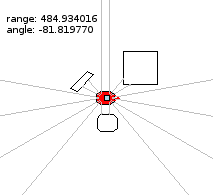
\includegraphics{sonarBot}
\end{center}
\caption{Sonar Robot Simulation}
\label{fig:sonarSim}
\end{figure}

\subsection{S-Curve Robot}

The S-Curve robot program was designed to move a robot through a curved
``canyon'' (see \figref{scurveSim}). An Action class was written to control the
heading of the robot so as to move parallel to the nearest object (a wall in
this case). At the start of the program the robot is commanded to move with a
constant forwards velocity and avoid hitting objects in front of it. This is
done internally by the Aria library which uses the wheel encoders to track its
velocity and its sonar range finders to detect object distances.

\begin{algorithm}
\caption{Set Heading to Follow Wall}
\label{al:folWall}
\begin{algorithmic}
\STATE get sonar reading (r,$\theta$)

\STATE side = $\theta < 0$ ? $1 : 0$
\STATE angle += $\theta + (2*side-1)*90$

\IF{angle $> \Delta\theta$}
	\STATE newHeading $+= angle$
	\STATE set Rotational Veloctiy = angle($.125)$
\ELSE 
	\STATE set Rotational Velocity $= 0$
\ENDIF

\end{algorithmic}
\end{algorithm}

\begin{figure}[H]
\begin{center}
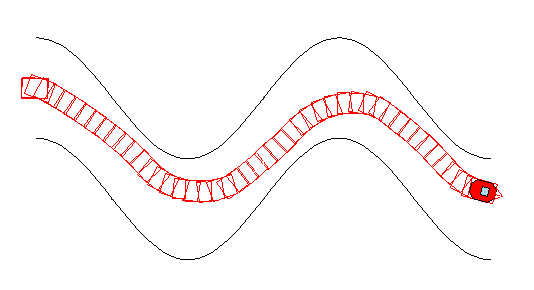
\includegraphics[width=.5\textwidth]{scurveBot}
\end{center}
\caption{S-Curve Robot Sinulation}
\label{fig:scurveSim}
\end{figure}


The robot monitors whether an object is in front of the robot at any distance.
If there is no object then the robot will not move. For this instance it stops
the robot once it reaches the end of the canyon. This is necessary for running
the robot in real time as to avoid having undesired behavior once it finished
following the curve. 

\alref{folWall} describes the method use to keep the robot parallel to the
walls. The robot needs to know which side the nearest object is on, and then
determine the angle to rotate so that it is normal to the wall ($\theta$ in
\figref{prWall}). Once the angle is known and it is outside of our threshold
value ($\Delta\theta$) then set the new heading and rotational velocity.

\begin{figure}[H]
\begin{center}
\usetikzlibrary{angles}

\begin{tikzpicture}[scale=3]
	\draw (0,1) -- (0,0);

	\begin{scope}[shift={(.5,.1)},rotate around={30:(.25,.4)}]
		\draw (0,0) rectangle (.5,.8);
		\draw[<->] (.25,1) coordinate (A) -- (.25,.4) -- (1,.4);

		\draw[<->,rotate around={-30:(.25,.4)}] (.25,1) coordinate (C) 
			-- (.25,.4) coordinate (B) -- (1,.4) 
			pic[pic text=$\theta$,draw,angle radius=1cm] {angle=C--B--A};
	\end{scope}

	\draw[->] (.75,.5) -- (0,.5) coordinate (D)
		pic[pic text=$\phi$,draw,angle radius=1cm] {angle=A--B--D};

\end{tikzpicture}

\end{center}
\caption{Angles For Parallel Wall Heading}
\label{fig:prWall}
\end{figure}

\end{document}
